\documentclass[12pt,a4paper]{article}
\usepackage[utf8]{inputenc}
\usepackage{listings}
\usepackage[toc,page]{appendix}
\usepackage{enumitem}
\usepackage{graphicx}
\usepackage{amsmath}
\usepackage{subcaption}
\usepackage{wrapfig}
\usepackage{geometry}
\usepackage{hyperref}
\usepackage{natbib}
\usepackage{amssymb}
\title{Review of Automation Techniques for the Assembly and Alignment of PIP-II Superconducting Cavities}
\author{Alfredo Bochicchio \\ Supervisor: Mattia Parise}
\date{October 2019}

\begin{document}

\maketitle


\begin{abstract}
\newline
    The report reviews state of the art technologies for automation both inside and outside Class 10 Cleanrooms, focusing specifically on the assembly and alignment procedure for SSR-I and SSR-II superconductive strings. \newline It reviews the entire spectrum of solutions for automation and metrology, with a focus on 3D machine vision solutions. It then presents the experimental setup and the results obtained applying a combination of 3D vision techniques to reconstruct and align two of the components of the string to achieve sub-millimiter accuracy. 
\end{abstract}
\begin{figure}[h!]
\centering
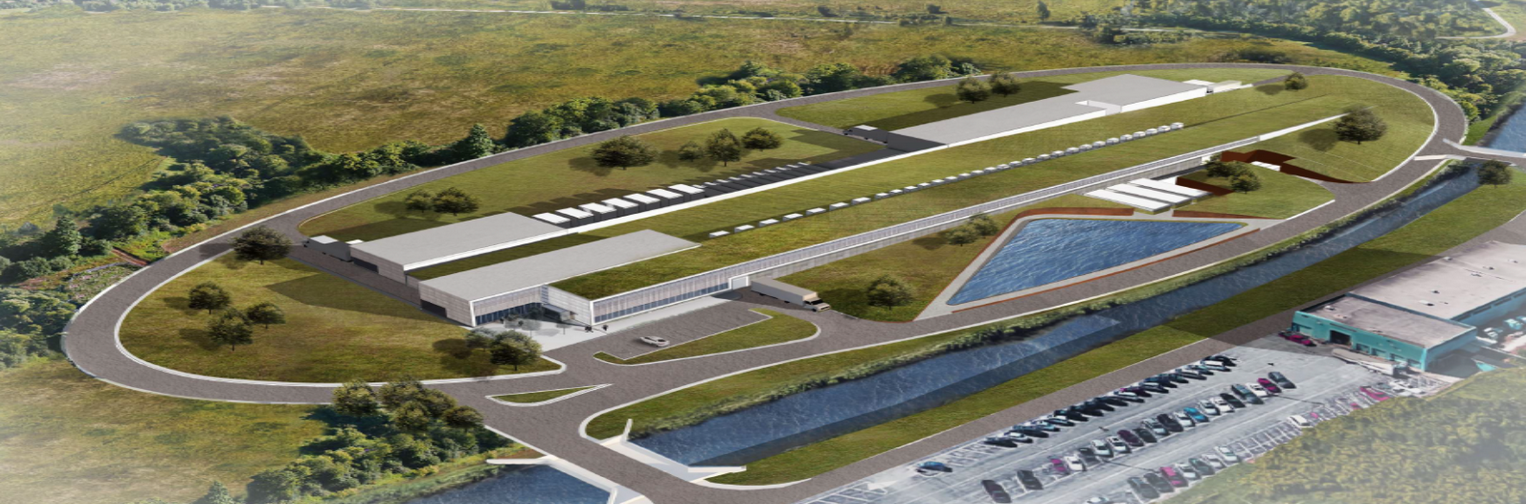
\includegraphics[width=1\textwidth]{1.png}
\end{figure}

\newpage




\section{Introduction}
\newline
PIP II is the new Proton Improvement Prorgram undergoing at Fermilab National Laboratory. It features a new brand 800-MeV accelerator that will replace the old Linear Accelerator updating the core technology to superconductivity. PIP-II will enable the most intense high-energy neutrino beam for the laboratory’s flagship project, the Long Baseline Neutrino Facility and Deep Underground Neutrino Experiment.
PIP-II is the first U.S. accelerator project that will have significant contributions from international partners, with Italy surely being one of the main contributors.
\newline
This document reports the work done by Alfredo Bochicchio during a 2 month internship at Fermilab National Laboratory. The broader aim of the project is to study how to introduce automation in the assembly process of the superconducting cavities for the new accelerator. The work is structured in the following way:
\begin{itemize}
    \item Part I: Review of the system, why automation is needed
    \item Part II: State of the art analysis of automation inside and outside cleanrooms 
    \item Part III: Proposed solutions for strings alignment
    \item Part IV: Experimental setup
    \item Part V: Results and consideration
\end{itemize}. 
\begin{figure}[h!]
\centering
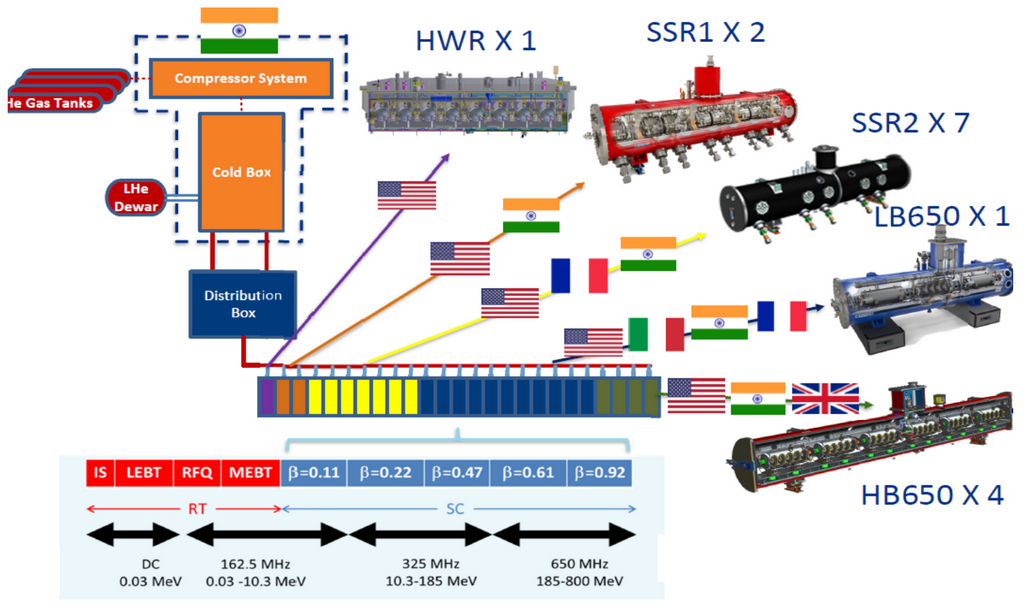
\includegraphics[width=0.75\textwidth]{20.png}
\caption{Overview of the modules of the New Linear Accelerator}
\end{figure}
\section{Overview of the Linear Accelerator}
The 215m long accelerator is composed of several modules which all work in specific energy ranges. \newline
I will focus mainly on SSR1 and SSR2 cryomodules. Each cryomodule is composed of 8 SSR Cavities (Single Spoke Resonator), 4 superconductive solenoids which act as focusing elements for the beam, and other mechanical elements that introduce compliance: the bellows.

\begin{figure}[h!]
\centering
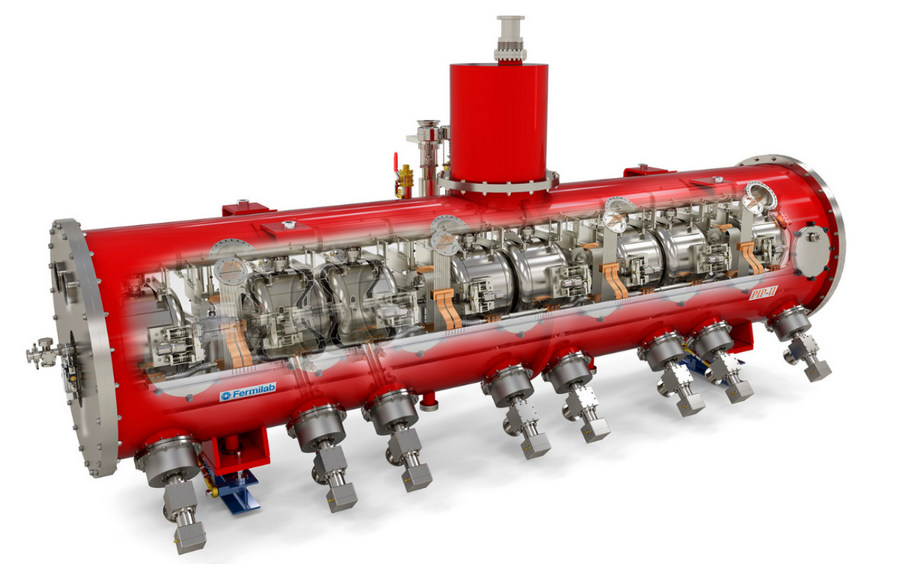
\includegraphics[width=0.8\textwidth]{23.png}
\caption{The SSR1 string}
\end{figure}

\subsection{The Assembly of SRF Cavities}
The process of designing and assembling Superconductive Resonant Frequency Cavities is complex and It involves several delicate operations often performed in extreme environments, such as Class 10 Cleanrooms.

\clearpage
\newpage

\subsection{Cleanroom Overview}



Cleanrooms are used in practically every industry where small particles can adversely affect the manufacturing process. They vary in size and complexity, and are used extensively in industries such as semiconductor manufacturing, pharmaceuticals, biotech, medical device and life sciences, as well as critical process manufacturing common in aerospace, optics, military and Department of Energy.

\begin{figure}[h!]
\centering
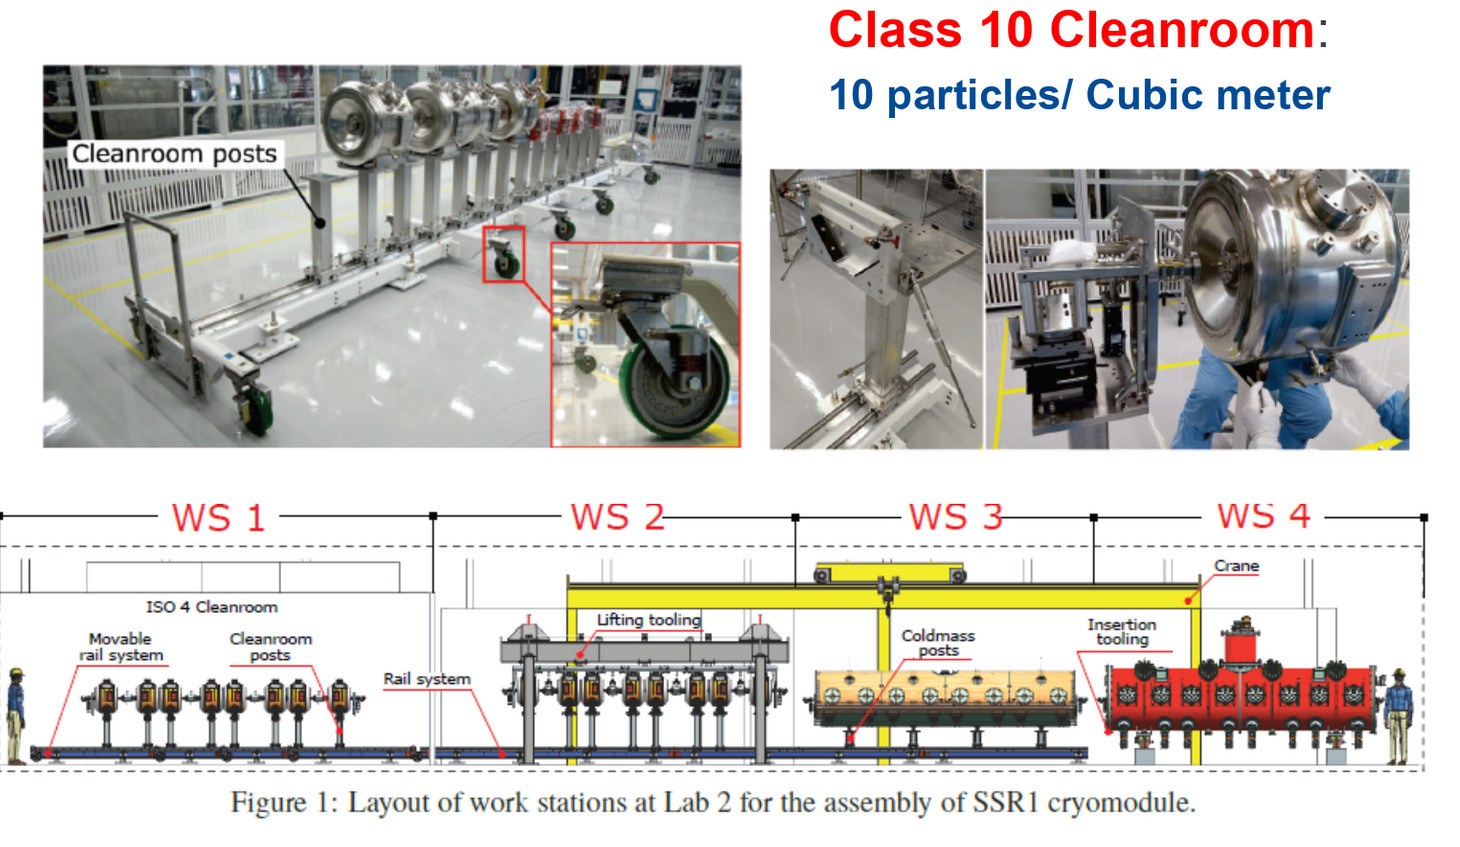
\includegraphics[width=1\textwidth]{4.png}
\caption{Top left: rails system for the cleanroom. Top right: Operations of the custom tooling. Bottom: Description of the procedure}
\end{figure}



In the entire string alignment and assembly procedure for SSR1 and SSR2 there is no automation. This cause poor and not repeatable performance. 
Part of the assmebly and alignment of the superconducting strings happens inside a Class 10 Cleanroom, which by definition has 10 particles of dirt over a threshold size per cubic meter. \newline


\clearpage
\newpage

\begin{figure}[ht]
\centering
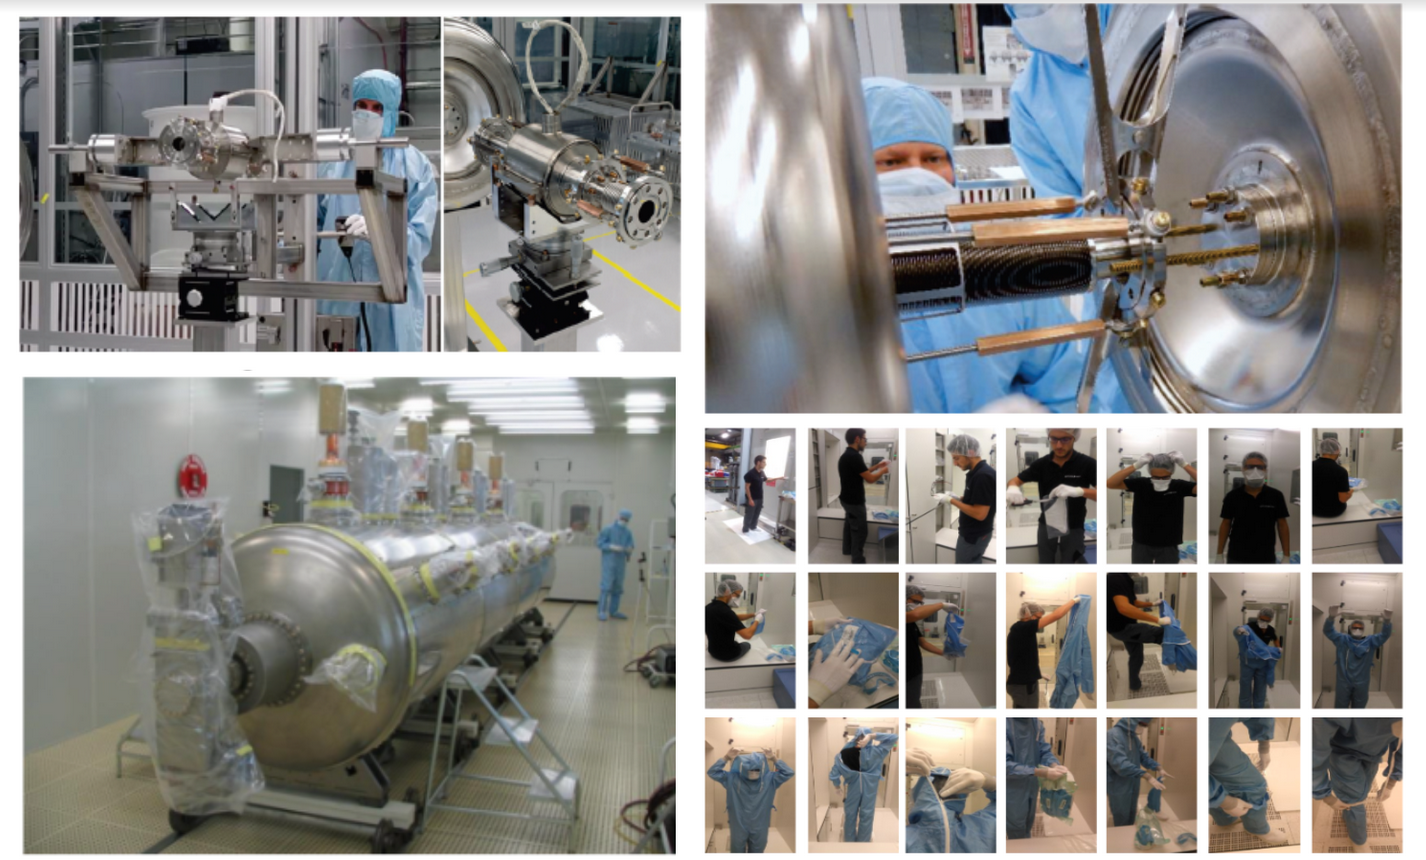
\includegraphics[width=0.8\textwidth]{5.png}
\caption{The long series of operations needed to enter and operate in the cleanroom}
\end{figure}


This means that a lot of expertise is needed to operate in such an extreme environment. The performance of the cavity is strictly related to the quality of the assembly procedure as any particle of dirt will deteriorate the performance.\newline 
By limiting the number and extent of operations that humans must do in the assembly process, we can boost the performance of the cavities and increase the repeatability of the process, ensuring a consistent improvement.


\clearpage
\newpage

\section{Analysis of Automation in Cleanrooms}
\begin{figure}[h!]
\centering
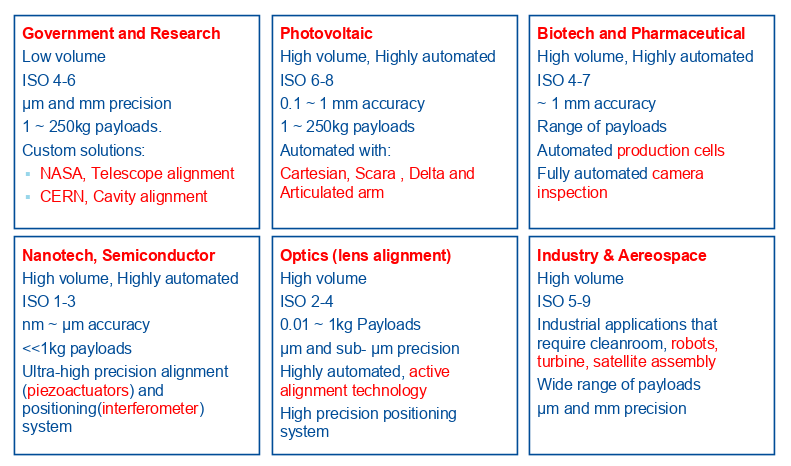
\includegraphics[width=\textwidth]{27.png}
\end{figure}

A wide range of industries are automating more and more their processes inside cleanrooms. 
Photovoltaic industry has similar payloads, standards and precision. However, that industry deals with high volumes which justify higher degree of automation in the manifacturing process. However, some of the cleanroom compatible manipulators, mainly Cartesian, Scara and Delta robot as seen in \cite{AutomationPhotovoltaic}, could be used in the string assembly process, either to align or to position components. 


%%%%%%%%%%INSERT REVIEW HERE%%%%%%%%
% A nice review of the characteristics of each manipulator can be found in.
Optics industry has nice solutions with respect to active alignment of lenses and other optical elements based on real time feedback (eg. \cite{Overview_of_Active_Vision_Techniques},
\cite{adaptive_measurement}). The concept of active alignment is surely fundamental for the the SSR1 alignment procedure. Other incredibly precise solutions have been used for research purposes: NASA has used micro and nanometer positioning systems (eg. Stewart Platform with piezoelectric actuators) for the alignment of the optical center of a modular lenses of a telescope.

\clearpage
\newpage


\subsection{Automation plan}

\subsubsection{Short Term: Active Alignment}
The Immediate solution would be to provide some assistive technologies based on active alignment. The easiest way would be to use either Cameras or Laser trackers to provide real time feedback.

\begin{figure}[h!]
\centering
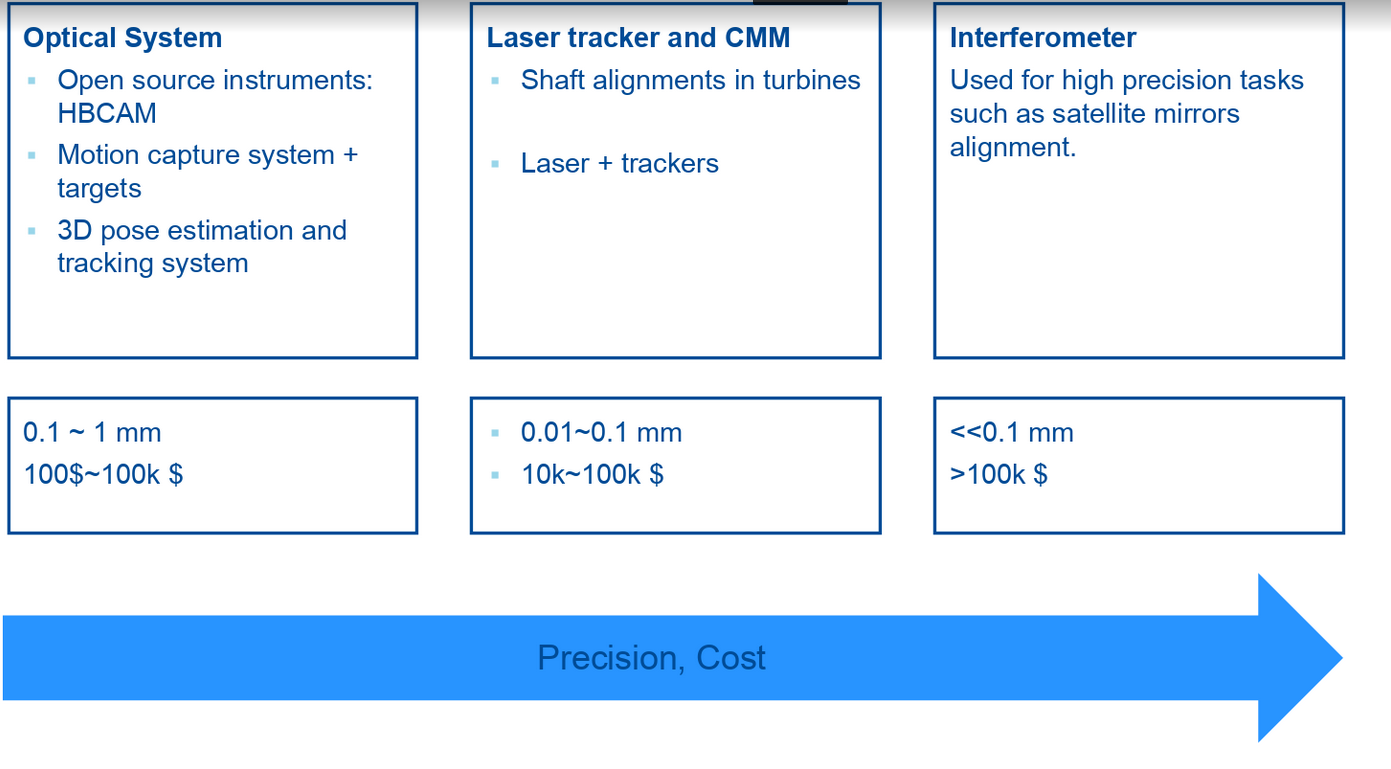
\includegraphics[width=\textwidth]{10.png}
\caption{Range of solution by cost and precision}
\end{figure}

Assistive technology must provide clear instructions to the operators. To do this we need to understand how the actuation of the micrometers affects the motion of the bellow. The custom tooling has L-R-L-R joints. We get the affine transformation from the Base frame to the End Effector just writing the DH Table for the tooling. However, the inverse problem must be solved:  How we reach a given pose in space by actuating the micrometers? There are many ways to solve the inverse kinematics problem. If the problem is redundant the analytical solution doesn't exist and there are other approaches to solve the problem, based on minimizing some value function. 

\begin{figure}[h!]
\centering
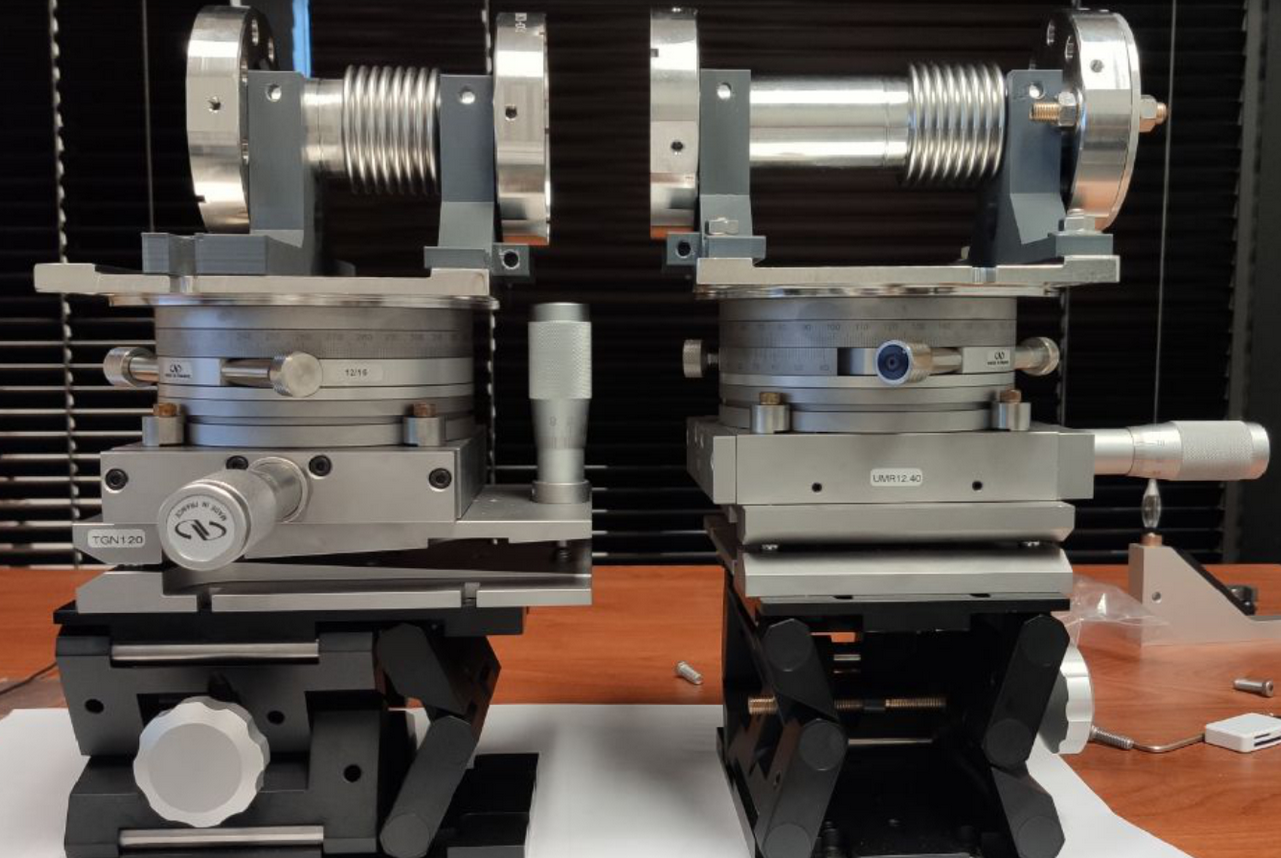
\includegraphics[width=\textwidth]{7.png}
\caption{The Custom 5 DOF toolings}
\end{figure}


\begin{figure}[h!]
\centering
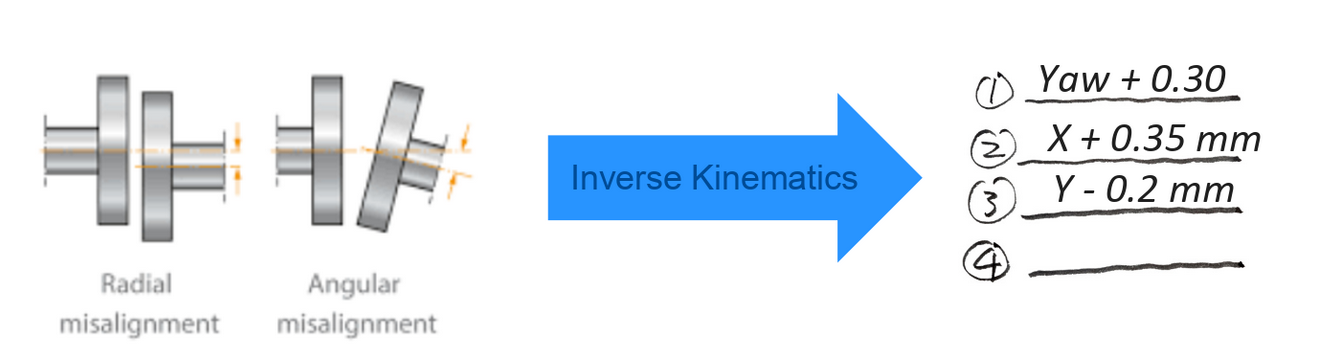
\includegraphics[width=\textwidth]{9.png}
\end{figure}
The set of clear instructions implies less operations, which translates in less sources of contamination for the assembly.



\newpage

\subsubsection{Mid Term: Semi Automation}
Class 10 cleanrooms have serious constraints on the materials that can be used inside. Traditional manipulators can't be used. However, there are many alternative. Each major manipulators company (ABB, Kuka) are starting to develop a segment specifically for Cleanrooms. While, given the production volumes at stake, it wouldn't make sense to adopt a high payload cleanroom compatible manipulator (250kg payload), but low payload manipulators could still be used efficiently, as they could actuate custom tooling that provide the necessary DOFs for the alignment. There are also cleanroom compatible mobile platforms that could help to move the low payload manipulator around. 

\begin{figure}[h!]
\centering
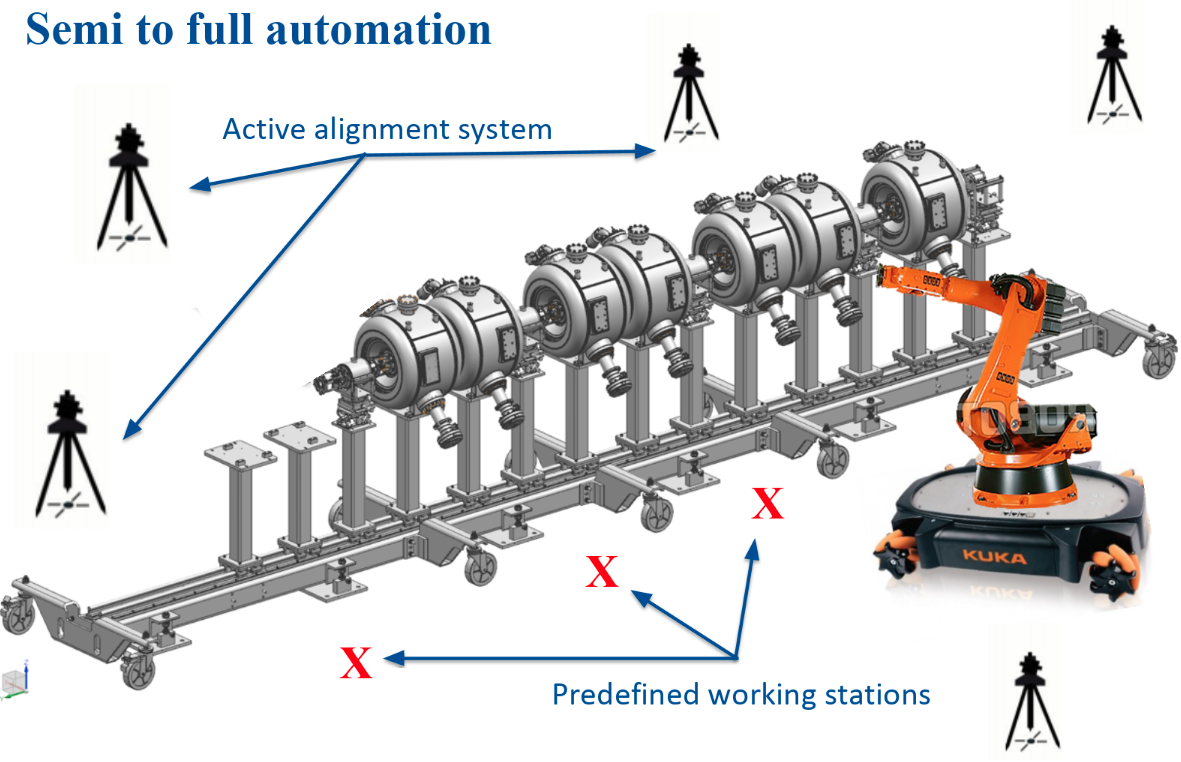
\includegraphics[width=\textwidth]{31.png}
\end{figure}

\newpage
\subsubsection{Long Term: Full automation}
Full automation would require no human intervention. The proposed solution is a pneumatic cleanroom compatible Stewart platform with switching rails to load every piece of the string on an active station that aligns them in the right position, ready to be assembled. This seems to be the best compromise between production volumes, price and quality improvement. The concept of a loading station may be infeasible or imply serious technical difficulties but the idea of a custom 5 DOF tooling still seems valid.

\begin{figure}[h!]
\centering
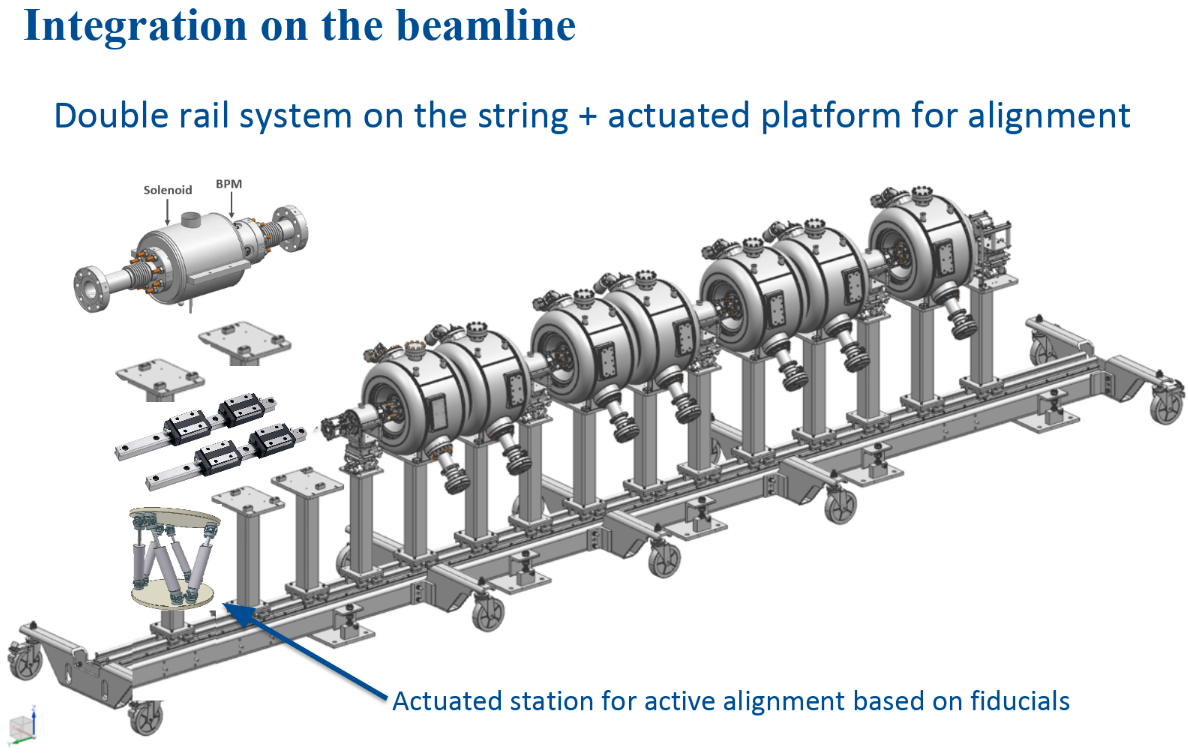
\includegraphics[width=\textwidth]{35.png}
\end{figure}


\clearpage
\newpage

\section{Solutions for Active Alignment}

While automation and manipulators would be used in the long term, in the short-mid term some hybrid solution is preferred. There is a wide range of possible solutions to provide real time accurate measurements to perform the active alignment.
\begin{itemize}
    \item Optical systems, HB-CAM, MOCAP and Multicam Setup
    \item Laser Tracker and Interferometer
    \item Coordinate Measuring Machine
    \item Optical Fiber
    \item Shaft Alignment for Turbines
    \item Projected Pattern
    \item 6D Pose with magnetometers

\end{itemize}

\subsection{Shaft Alignment for Turbines}
These solutions are used for aligning turbines shafts axially. They are incredibly fast and cheap, however they require a lot of components to be mounted axially on the  cavities and require some space to be mounted, which ultimately means more contamination and less performance for the module.

\subsection{Interferometer and Laser Tracker} 
This is the most precise solution, as laser tracker can resolute up to micrometers and milliradians as shown in \cite{Laser_triangulation}.
 The price range is 10-100k \$, which would be a good compromise for their performances. However, the setup must be carefully calibrated, placed and operated. They could monitor the alignment really well but they are not ideal in a cleanroom, consisting in many different parts.

\subsection{6D Pose with magnetometers}
This solution consist in an array of 1D magnetometers that are able to triangulate the pose of a magnet in 3D space. A detailed version is presented in: \cite{magnetometer}. They have been used in prosthetics hands and other similar devices, as they are very small and require low power. However, they are still physical objects that must be placed and referenced with respect to the string components. Moreover, the technology is based on electromagnetism, which is not ideal near strong electric and magnetic fields.


\subsection{Optical Fiber Shape Sensing}
It is well known however that optical fibers can measure strain very accurately, up to micrometers of strain. The core technology is Fiber Bragg Grating sensors, which consists in equally spaced features of the cable that reflects specific wavelengths. When they are subject to a strain the reflected wavelength is shifted. One fiber can have multiple of this sensors by reflecting different ranges of wavelength. They are actually used in structure health monitoring, railroad monitoring, and in other applications where distributed sensing is required. The resolution is extremely good and it could very well be used to monitor the alignment of the string assembly once it is assembled.
Other technologies that exploit the same principles are able to reconstruct the shape of the fiber in 3D (\cite{fiberopticsshapesensing}), thus monitoring every relative displacement. I didn't consider this technology as It may still have a low Technology Readiness Level, but It is worth to consider.

\subsection{Coordinate Measuring Machine}
The CMM is currently being used to reference the pieces with a very high precision (micrometers). It doesn't have a big work volume and it is obviously not compatible with the cleanroom, however it still provides the best accuracy you can get to measure positions, targets and shapes. 

\subsection{Optical Systems and Projected Patterns}
Computer vision is becoming more and more popular. This because it is a relatively simple, modular and versatile solution. It is easy to implement low budget solution to demonstrate the feasibility of some techniques and then scale the system to obtain the necessary performances.
An example of how computer vision has been used for metrology and accurate measurements is the HBCAM system.
It consist in multiple cameras with a laser light source and some reflective targets. These spherical targets are mounted in accurately machined metal frames so that the position of the targets is known with great precision.
By mounting these frames on the components and accurately referencing them with a CMM, you can monitor the alignment of the strings just by looking at the relative position of the targets.
This system however, has many limitations: the frames have metal structures that must be mounted on the pieces, this require to perform a lot of manual operations, making it incompatible with the clenaroom.
Another optical system to consider is the MOCAP (Motion Capture System), or more in general, a Multi Camera Setup. These are usually setup of 8-24 Cameras that are able to monitor markers inside a work volume of several cubic meters. They can get to mm and sub mm accuracy, however they generally are thought for high speed movements, and they usually need a lot of setup / calibration and they need physical markers. It would be ideal if we were able to use this system without markers, just using 3D computer vision techniques or non physical targets, such as known projected patterns, from which we can extrapolate the information on the object pose.


\subsection{Excursus of Computer Vision Techniques}
More information on the use of computer vision techniques can be found in Halcon manuals \href{https://www.mvtec.com/products/halcon/documentation/}{(link)}. This is only a brief overview of possible handy use cases.
\begin{itemize}
    \item Inspection and Quality assesment
    \item Measurements
    \item 3D Reconstruction
    \item Data and information retrieval
\end{itemize}

\subsubsection{Inspection and Quality Assesment}
For this task special telecentric lenses are used. This lenses do not have any (ideally) distortion and do not deform the real world image by introducing a perspective transformation. With such systems you can easily analyze real world shapes and inspect surfaces. Defects can be found by training neural networks on huge datasets of labelled examples of pieces with and without defects. 
\subsubsection{Measurement}
Any kind of 2d and 3d measurement can be taken with the appropriate optical system. Resolution of the measures can scale with the system. There is an enormous variety of techniques. Model based techniques do exploit prior knowledge of the shape (\cite{munoz_fast_2016}) Light based techniques use deformation of known and carefully calibrated light patterns to infer the position of world points. Measurement is strictly related to reconstruction.
\subsubsection{Reconstruction}
Also here there are several techniques, Model Based, Shape Based, Deep Learning techniques, Stereo Vision, Sheet of Light, Depth from Focus, Photometric stereo vision.
The concept is all the same, in order to reconstruct the 3D object more then one perspective is needed, and among all this perspectives there must be matching features in the images such that an algorithm can reconstruct the XYZ coordinates of such features. If the object is featureless or homogeneous some projected pattern is needed.

\subsubsection{Data retrieval}
Cameras can read any kind of data, both structured and unstructured. Text, Bar code, labels, even object classification and recognition can be automatized with many algorithms such as the famous OCR for text recognition. They have reached impressing levels of accuracy, and they can be very useful in limiting the quantity of information that human operators must deal with. This is usually combined with Virtual Reality or Augumented Reality, especially in the automotive industry, where workers are guided in complex procedures to limit the probability of errors.  
\begin{figure}[h!]
\centering
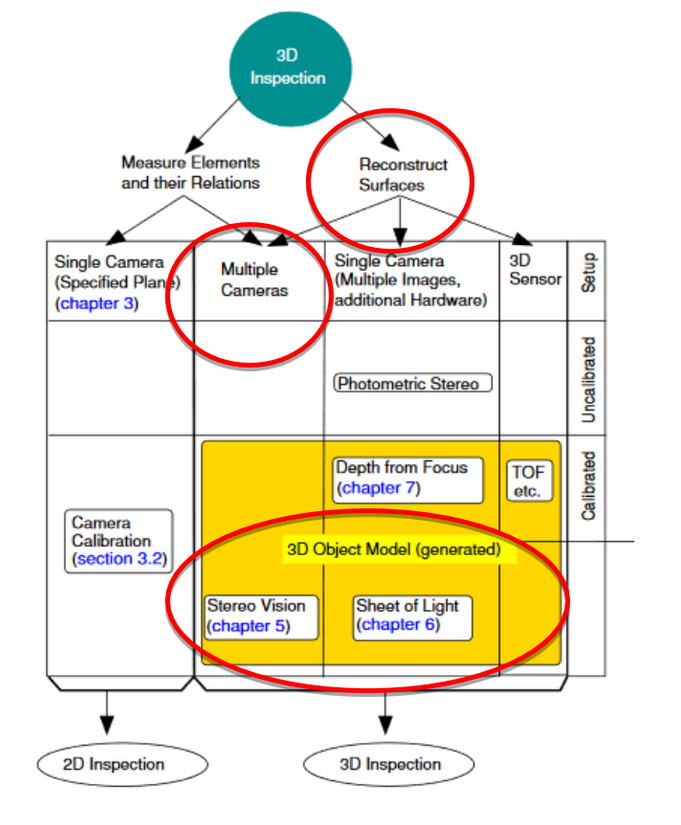
\includegraphics[width=\textwidth]{12.png}
\caption{In red, the best choices for solving the reconstruction and alignment problem: Surface reconstruction with a multicam setup to obtain a 3D object model, which is used either for Model Based pose estimation or Point Cloud Alignment algorithms}
\end{figure}
\clearpage


\newpage
\section{Experimental Setup}
The purpose of the activity is to study and evaluate some of the existing techniques to actively monitor the aligment of SSR1/SSR2 strings.
The experimental setup consists in:
\begin{itemize}
    \item Two custom 5 DOF toolings
    \item Two bellows that must be aligned.
    \item The Zed Stereo Camera
    \item Custom CNC frame for XYZ positioning of the bellows. 
    \item A green 5mw laser projector
    \item An optical setups to focus and modify the shape of the laser
\end{itemize}
\begin{figure}[h!]
\centering
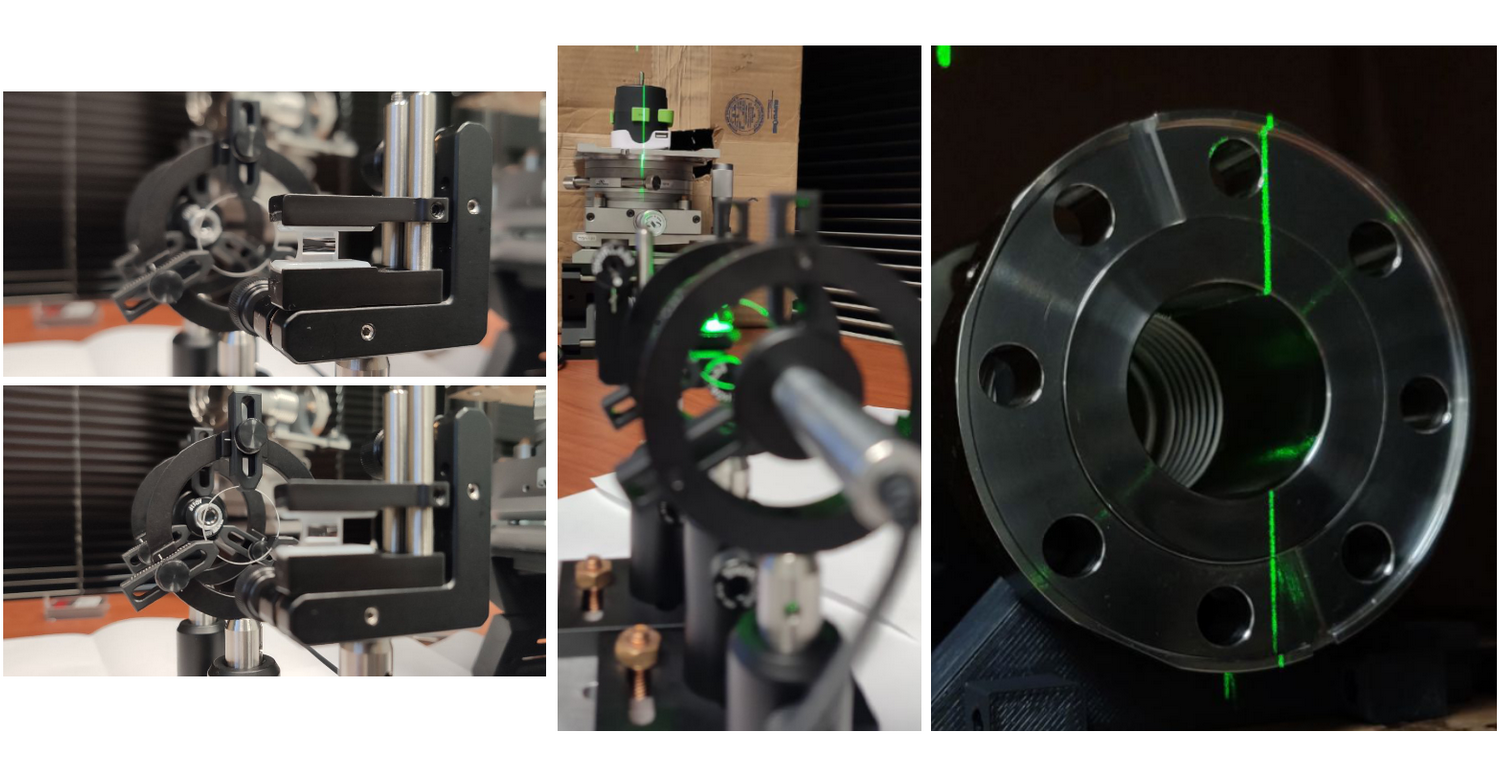
\includegraphics[width=\textwidth]{15.png}
\end{figure}
I have chosen to use a stereo camera setup with computer vision techniques as It seems to be the easiest to experiment with, and possibly the cheapest solution on the market with a precisionup to 0.1mm if everything is done accurately.


\subsection{Camera Calibration and Measurement accuracy}
The first step when using computer vision to measure is to calibrate accurately the camera. It can be done in many ways, and not all of them are equivalent. Some good metric to evaluate how good is the calibration is the average re-projection error. Camera calibration rely on many photos of a known geometrical pattern and It finds the parameters of a polynomial that transforms the known pattern into the observed pattern.
In order to achieve precise measures with a Stereo Camera, which means the z coordinate of world points, I must accurately esteem the disparity, which is distance between the coordinates of the same world point in the two image planes.
To compute the disparity, there are algorithms that are able to estimate the position of a world point with subpixel accuracy. The chessboard corners for example are esteemed with subpixel accuracy by computing the highest point in the gradient function. The subpixel accuracy in the disparity estimation can make the big difference between cm and sub-mm accuracy as also seen in \cite{sub_pixel_laser_spot}
\begin{figure}[h!]
\centering
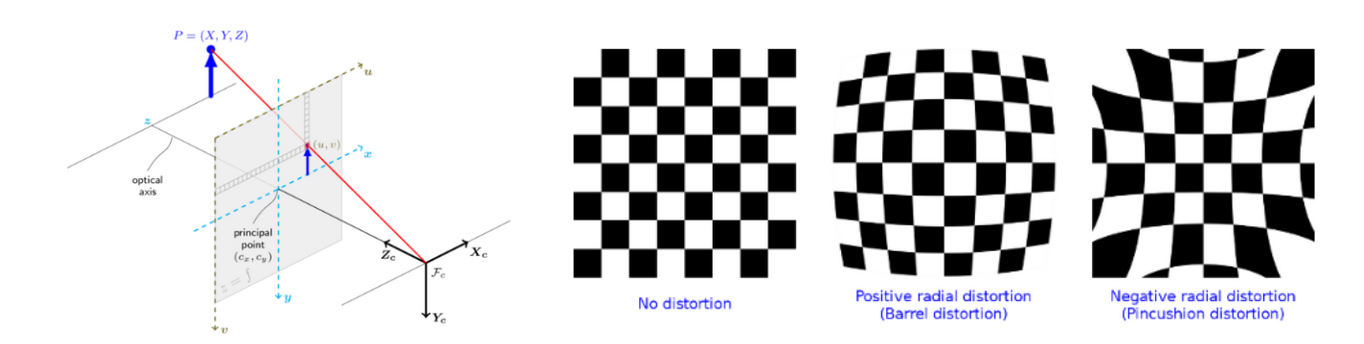
\includegraphics[width=0.8\textwidth]{11.png}
\end{figure}
I was able to reconstruct the world position of a point with an accuracy of 0.15mm which is reasonable for the alignment task. The relative precision on rotation is much more complex to define. One way would be to compute the difference between the module of the quaternions that describe the rotation. I avoided the problem by estimating the rotation from world points of known relative coordinates. A complete error model for the Zed stereo camera can be found in \cite{Zed_data_error}

\subsection{Sheet of Light \& Stereo Sheet of Light}
\begin{figure}[h!]
\centering
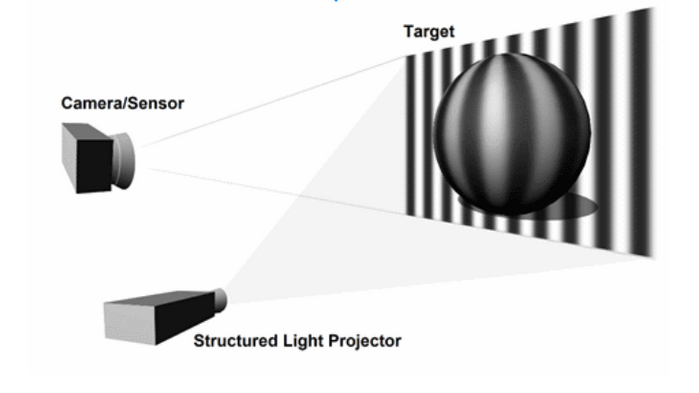
\includegraphics[width=0.8\textwidth]{13.png}
\caption{Sheet of light setup with Camera and Laser}
\end{figure}

The previous results show that the desired accuracy in the alignment can be reached. The ideal solution would not make any use of physical targets, as they require some effort to be introduced in the clean room and mainly, they need to be referenced with a Coordinate Measuring Machine. That is why solutions based on light and projected patterns \cite{zhang_online_2017} are effective. 

% \begin{figure}[h!]
% \centering
% 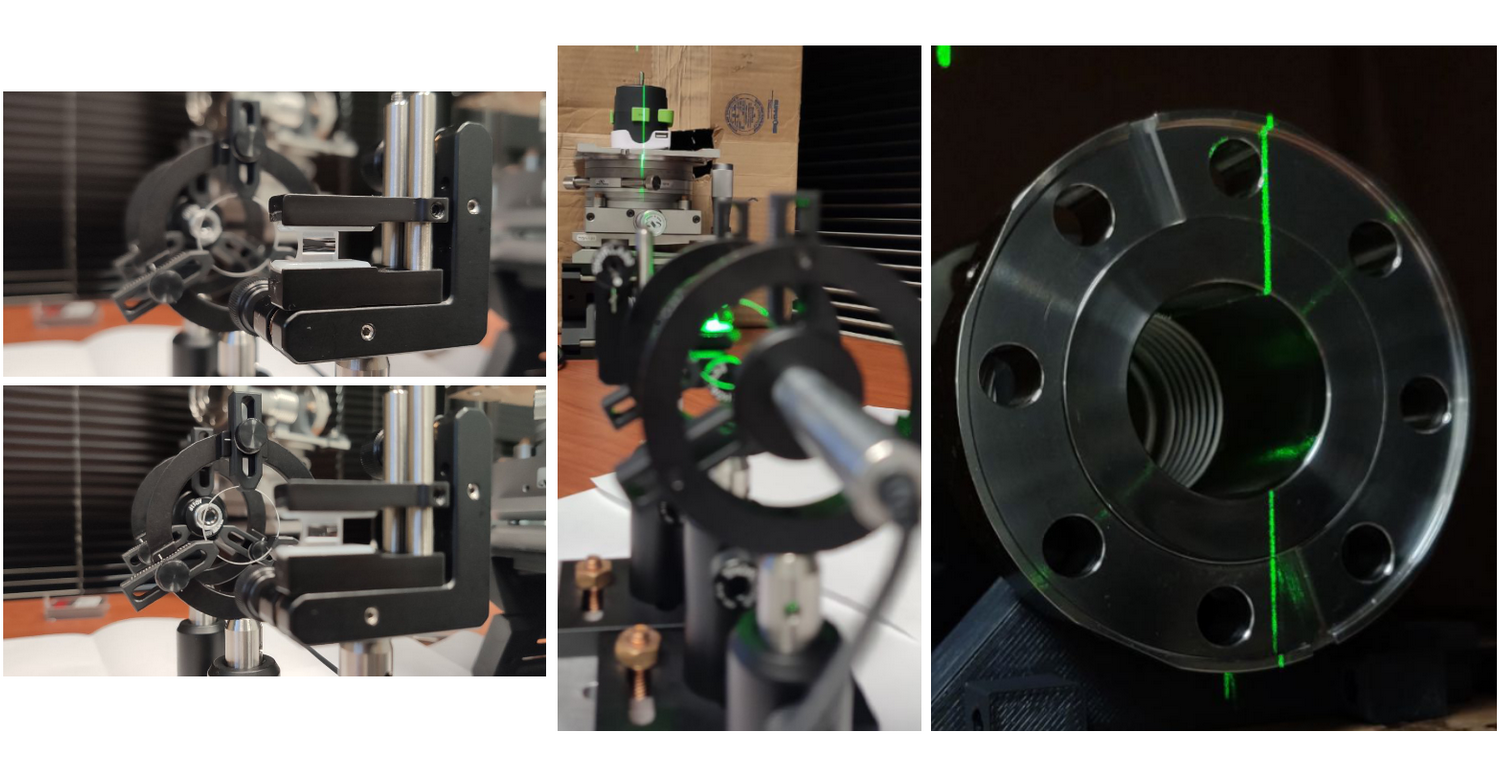
\includegraphics[width=\textwidth]{15.png}
% \end{figure}
 In normal sheet of light, you know through calibration the relative position of a line light source and the camera. When the line is projected on some irregular surface it is distorted. If you compute the difference in position from where the light is projected and where it should be if there was no object you are able to precisely reconstruct the 3D points that belong to the object's surface. By doing this on the entire object you are able to reconstruct the entire surface. Many working examples are found in the literature such as 
\cite{3d_scanner_structured_light} and 
\cite{3d_structured-light_scanner_2019}
 \begin{figure}[h!]
\centering
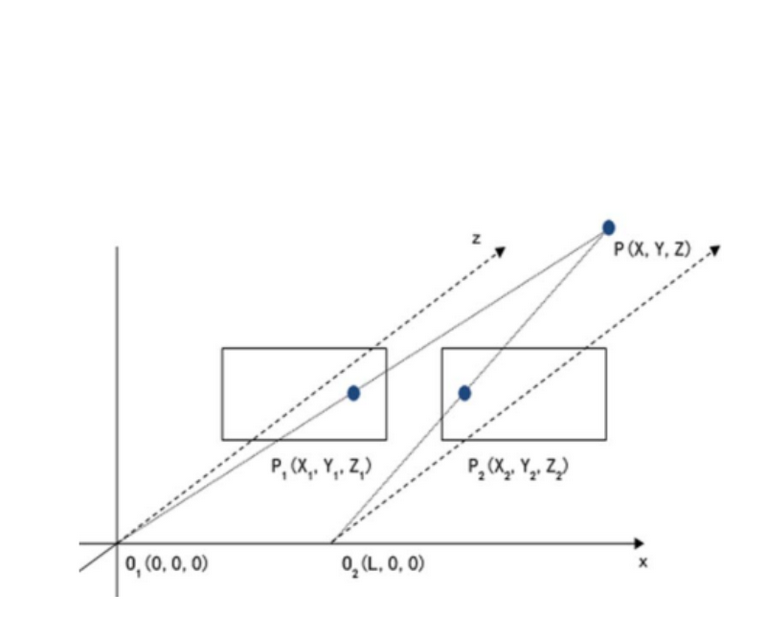
\includegraphics[width=0.7\textwidth]{14.png}
\caption{World coordinates from disparity map}
\end{figure}
The stereo sheet of light technique has the only modification that it doesn't need to be calibrated as it computes the Z from the disparity map of the two cameras.  The problem then becomes matching the same pixel in left and right image plane. There are several ways to match points, and most of them are based on feature detection. However, that doesn't necessarily work with a featureless object, and niobium cavities do not have many features to detect. If you use projected pattern or laser line the matching problem is solved if some assumptions are made. The assumption in my case is that image plane and laser line plane are perpendicular, which means that every pixel in one image will have the correspondent pixel in the same row of the image plane.


\section{3D Model reconstruction}

\begin{figure}[h!]
\centering
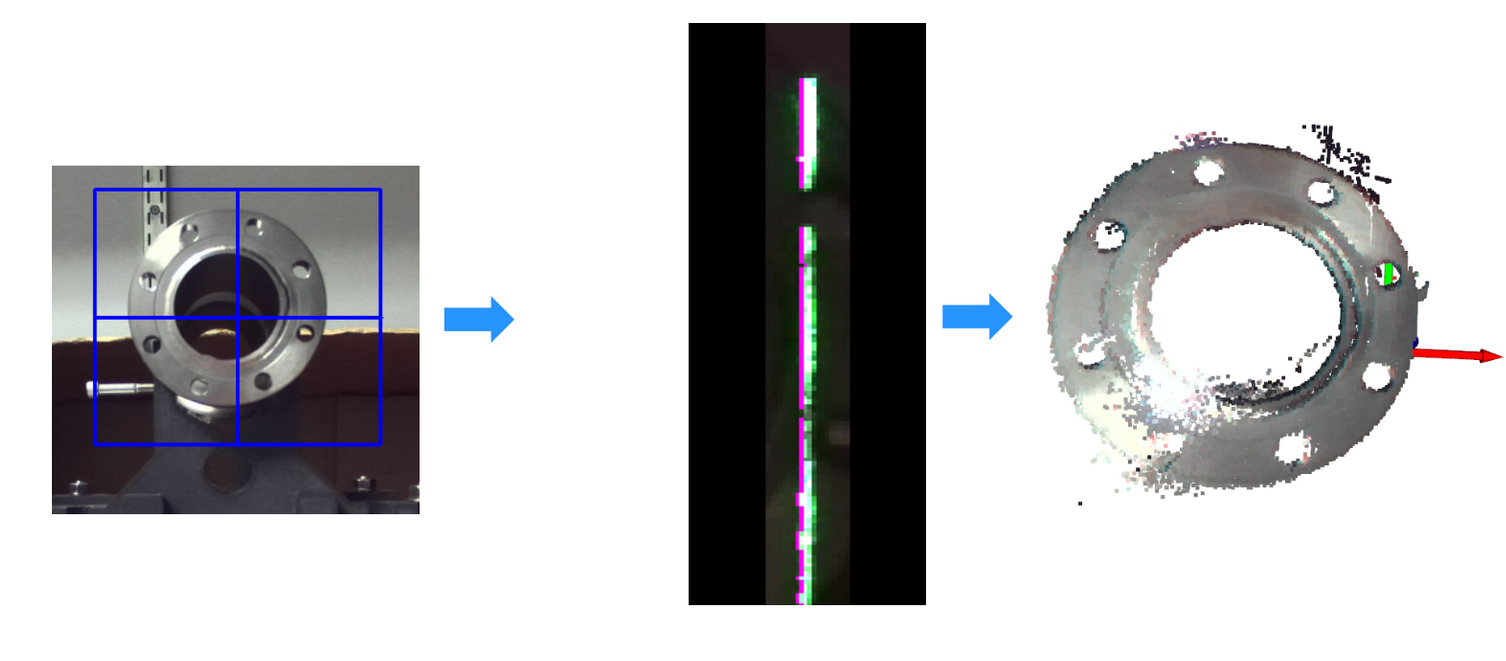
\includegraphics[width=\textwidth]{17.png}
\end{figure}

\subsection{Workflow of the 3D scanner}
I have implemented a 3D realtime scanner with Python based on the work of \cite{Binocular_3d_scanner} and \cite{ulrich_engineering_2019-1}. The workflow is described accurately in the github repository. I first acquire the image with a stereo setup. Then I project a green laser line on the object, and i extract the center of the line both in left and right image. I calculate the center with subpixel accuracy by averaging the gradients of the lightness and intensity of green. 

\clearpage
\newpage

I then use the disparity to calculate the world coordinates of corresponding points. By repeating this process over the whole object I am able to reconstruct the object in 3D. This process outputs a Point Cloud, which I can use to reference targets, measure, and check for defects and other imperfections.

\begin{figure}[h!]
\centering
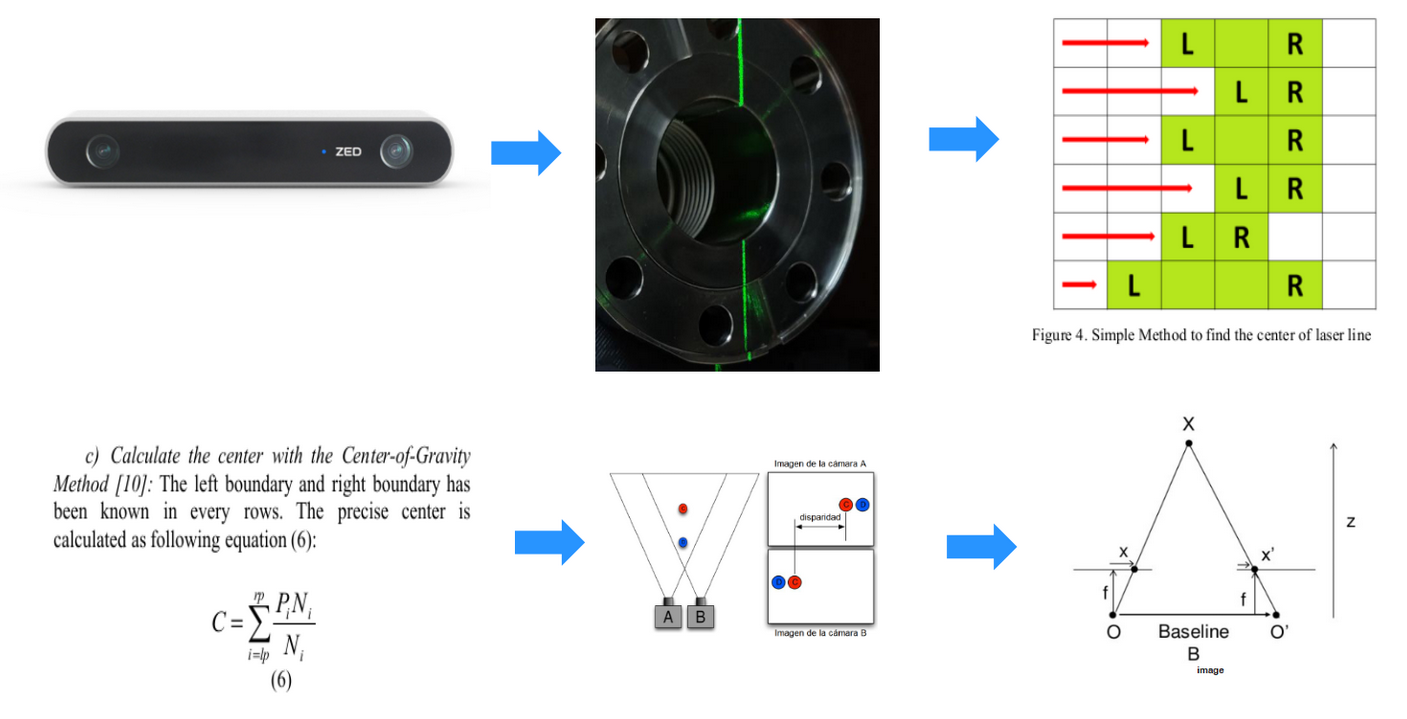
\includegraphics[width=\textwidth]{16.png}
\caption{a) Zed Camera b) Laser line on the object c) Laser line extraction d)Subpixel laser line center e) Disparity Map f) World coordinate reconstruction}
\end{figure}


\clearpage
\newpage

\subsection{Reverse engineer with point clouds}
Once you have point clouds you virtually have a CAD model of the object. However, there are a lot of steps that can increase the quality of the model. The original point cloud will have a lot of noise, and there are algorithms for outliers detection and removal. Moreover, multiple point clouds of different views have to be fused in one model. This is done by aligning at least three points manually and then running algorithms that minimize a distance metric iteratively.
\section{Results}
The 3D laser scanner works very well on uniform plastic materials. It is able to reconstruct object with high precision. It work less well on shiny surfaces, such as steel and niobium. 
The two main problems where extracting the subpixel position of the line center are:
\begin{itemize}
    \item In-camera reflections
    \item Laser Speckle
\end{itemize}
In-camera reflections are hard to eliminate as for circular objects there will always be a point along the radius that is reflecting in camera. Reflections can be locally eliminated by carefully adjusting the exposure and brightness, however this is a very tedious work which hasn't been automatized yet. Very good automation is found in traditional sheet of light techniques, as there are powerful libraries for light stripe extraction (\cite{he_study_2003}, \cite{hoiem_maximize_2018}) The problem with the merging is that being axially symmetrical I do not have any reference to merge points. This could be solved since the point cloud is RGB and some colored markers can easily be matched with this procedure.

\section{Techniques for 3D Pose estimation}


\subsection{Multi correspondence: Point Cloud Alignment}
The output of the stereo sheet of light technique is a point cloud. If I am able to align the models of the objects, I will then have a reference for my point clouds. If I found the transformation that align the bellows with the aligned bellows I can just enforce that transformation with inverse kinematics and i reach the goal.
There are many algorithms that can align clusters of points. There are many implementation, but for this problem I suppose that we are trying to find the rigid transformation that minimize the error (average distance) between two point clouds. If we are able to produce a real time point cloud of the object, we may be able to find the transformation between the real and the aligned bellow to understand the transformation, and by inverse kinematics also the actions that are needed to align the bellow.
I have tested many of this algorithms for point cloud alignment. There are fully working versions already implemented in PCL (Point Cloud Library), and Matlab (CPD and others).
The system works if I manually misalign the CAD model, but is still not able to match the scanned point cloud of the bellow with the CAD one. 
The problem with the Steel and Niobium cavities is that the quality of the point cloud is not sufficient to perform the alignment. I was able to test this the performance of the algorithm by using the Cad Model to generate random downsampled set of the original point cloud and see if I was able to reconstruct a known transformation with these methods (CPD, PCD). The results were eccellent, but they must still be tested with the scanned point cloud instead of the CAD generated one.
\begin{figure}[h!]
\centering
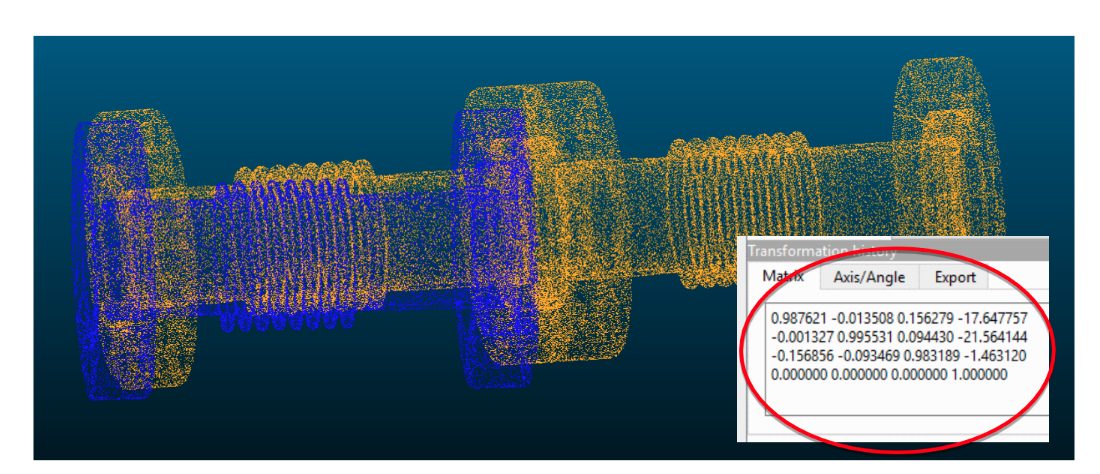
\includegraphics[width=\textwidth]{36.png}
\end{figure}

\newpage

\subsection{Model Based Pose estimation}

The chosen technique for 3D pose estimation in the end was 3D shape based matching and it is a model based approach, as It needs the CAD model or the reconstructed model of the object.
The concept is the following:
It first extracts the edges of the CAD model with a CANNY filter, which computes directional gradients of the image. It then create a pinhole camera model with a perspective, which is the model obtained from camera calibration. Given the perspective models it calculates how the edges would appear from different points in space. The XYZ points of the edges are transformed in image plane coordinates through the camera matrix. When you present the algorithm with an Image, it extracts how the edges appear in the image and calculate the point in space that, given the perspective, gives the closest matching edges, and it is based on a minimum error criteria. The algorithms has to calculate and store how the edges would appear from different point in space, with an high resolution. This means that you must give a good initial guess of the relative pose so that the stored model can be as small as possible.
I found an implementation of this algorithm in the HALCON software, which has a lot of other useful implementations almost ready to use. However, there are many open source implementation of the algorithm which can be found on github, but many of them are less polished or less robust versions.


\subsection{Model Based Pose estimation precision}
The precision highly depends from how well the algorithm is able to extract corners from the image. The sharper and more identifiable the geometry of the object is, the better the result would be. The cylindrical symmetry of the cavities is bad for the algorithm, as it can't distinguish the rotation except for the side holes. The precision is around 1mm which is not enough, but can easily improve if the model based estimation is done with more criteria, which means better lightning, uniform shadows and other common sense practices that improve edge extraction. However, the feedback can still be used to align two components using a custom positioning setup.

\subsection{XYZ Setup for Alignment}
In order to experiment with the alignment, We built a 3 DOF positioning system with 3 linear motors and rails from a CNC printer. The motors need dedicated power supply and motor controller, however they easily interface with Arduino and Simulink. The goal was to align a bellow to another bellow by positioning the component in 3D based on the active feedback from Model Based Pose estimation. All the elements are working, but the integration of the whole system needed few more days to setup.
\section{Tools}
There are many options: 
\begin{itemize}
    \item Matlab CV Toolbox : 
    \item OpenCV : Most used open source computer vision library. Available in C++ and Python. It has a loot of useful tools and features implemented. 
    \item Halcon MVTech : Halcon is the emerging software for ready to use computer vision solutions. It has a lot of documentation and seems to be quite immediate to learn. 
    \item Open source packages for Model Based pose estimation developed at Arizona State University by professor Ben H. Amor. , as well as other Deep Learning Packages for Hybrid Model Based estimations.
\end{itemize}
Matlab has a lot of functionalities already implemented, and if you find the right toolbox It increadibly speeds up the process. However, there are some restriction eventually, and less freedom to operate with dedicated software from Cameras. Matlab in fact wasn't able to interact with the ZED camera to directly modify the exposure and shutter speed (unlike Python, \cite{noauthor_zed-python-api/tutorials_nodate}
), which is a serious limitation when having to adjust parameters for in camera reflections. OpenCV and C++ or Python are extremely versatile solutions (eg. \cite{slr_camera_Python}, \cite{out-sider_cheap_2018}
), anything can be done , however being open source they require more effort to implement slightly new algorithms. A lot of pre made repositories can be find on github but there is usually a lot of work to integrate other's solution in your system. 


% \subsection{Measurement accuracy}
% The purpose of the early work was to demonstrate that it is possible to achieve sub-millimeter precision with a commercial setup (100\$-500\$).
% To perform accurate measurements you need a proper calibration. You have many options, all of them are quite valid. As we are trying to "push" the limits of measurement accuracy (usually you get mm precision out of this measures with an average setup) there are a number of things you must look for. The calibration pattern must be as precise and straight as possible, possibly glued to a stirofoam or some other rigid support. In the calibration phase, you must make sure that your pattern was photographed in many different poses, making sure that you don't leave area of the frame uncovered. 
% There are some metrics to evaluate the precision of a calibration, such as the reprojection error, that can be quite useful in evaluating the precision you can get out of a calibrated camera.


% \subsection{3D Reconstruction}
% A hot topic in Computer Vision is 3D reconstruction. The possibility of real time reverse engineering on the object in your hands. You can scan It to automatically find defects, to extrapolate properties and, ultimately, you need the model to align it. Model based pose reconstruction in fact is much better and faster then just pose reconstruction.
% There are many possibilities to do 3D reconstruction. I chose stereo sheet of lights techniques. First of all, it is very easy to implement. You just need a stereo camera setup, and no need for calibration at all. You just make the assumption that the plane 

% Cit. Paper.
% Why I 

% \subsection{Pose estimation}



\clearpage
\newpage


\section{Conclusion}
This report could just be the beginning of a long term project whose goal is to increase the performances of cavities by ensuring more repeatable procedures. The work tries to provide a broad picture of the existing technique to automate some aspects of the SSR1 and SSR2 assembly process. 
\newline
The experimental work demonstrates that it is feasible to develop in relatively no time and limited effort systems that can be scaled up and adapted to solve real problems and tasks.

\newline

\newline
Computer Vision solutions proved to be extremely cheap and versatile while still being effective. The precision and accuracy should be good enough to perform the alignment task, and the system can be effectively scaled up to have much larger work volumes. It could be useful both inside and outside clean rooms to align and monitor the assembly. Active alignment is fundamental in the short term automation phase, and the best solutions are systems that exploit lasers and light patterns without using any physical targets, which can be sources of contamination inside the cleanroom. The easiest setup which doesn't need calibration, Stereo Sheet of Light, proved to be a bit fragile with all the in-camera reflections. Model based estimation on the other hand, is extremely reliable, and its performance could be enhanced by using some Deep Learning Framework and training on the components of the cavity.







\clearpage
\newpage




\bibliographystyle{plain}
\bibliography{ref}




\end{document}
